\begin{enumerate}
    \item The hour-hand of a clock is $6 cm long$ . The angle swept byit between $7:20 a.m.$ and $7:55 a.m.$ is:
    \begin{enumerate}
    \item $ \left(\frac{35}{4}\right)\degree $
    \item $ \left(\frac{35}{2}\right)\degree $                                
    \item $ 35\degree $                  
    \item $ 70\degree $  
    \end{enumerate}

\item In the given figure, the quadrilateral PQRS circumscribes a circleHere PA + CS is equal to:  
\newpage
	\begin{figure}[!ht]                                    
    \centering                                            
    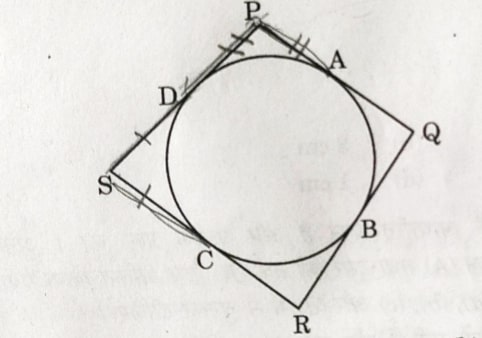
\includegraphics[width=\columnwidth]{figs/ct1.jpg}      
    \label{fig:image2}                                      
    \end{figure}  
    \begin{enumerate}
    \item $ QR $
    \item $ PR $                                          
    \item $ PS $                                          
    \item $ PQ $
    \end{enumerate}  




    \end{enumerate}

